\documentclass{beamer}
\usepackage[utf8]{inputenc}
\usepackage[T1]{fontenc}
\usepackage{eurosym}
\usepackage{rotating}
\usepackage{comment}
\usepackage{tikz}
\usepackage{pgf-umlcd}
\usetikzlibrary{arrows,automata,shapes}
\AtBeginSection[]
{
  \begin{frame}
  \frametitle{Wir sind hier:}
    \tableofcontents[currentsection]
  \end{frame}
}

\begin{document}

\title{Erkennen eines Graphen aus einer Punktwolke}
\date{}

\frame{\titlepage}

\section{Einleitung}
\frame{\frametitle{Das Problem}
\begin{description}
\item[Eingabe] ein metrischer Raum $(X, d)$, z.B.
  \begin{enumerate}
  \item GPS-Koordinaten eines Autos, das in einer Stadt herumfährt
  \item Koordinaten der schwarzen Pixel in einem Schwarz-Weiß-Bild
  \end{enumerate}
\item[Ausgabe] eine Approximation des metrischen Graphen, der dem metrischen Raum zugrunde liegt, z.B.
  \begin{enumerate}
  \item das Straßennetz der Stadt
  \item der Graph, der im Bild abgebildet wird\\ $\rightarrow$ Schrifterkennung
  \end{enumerate}
\end{description}
}

\frame{\frametitle{Beispiel (Erdbeben)}
\begin{figure}
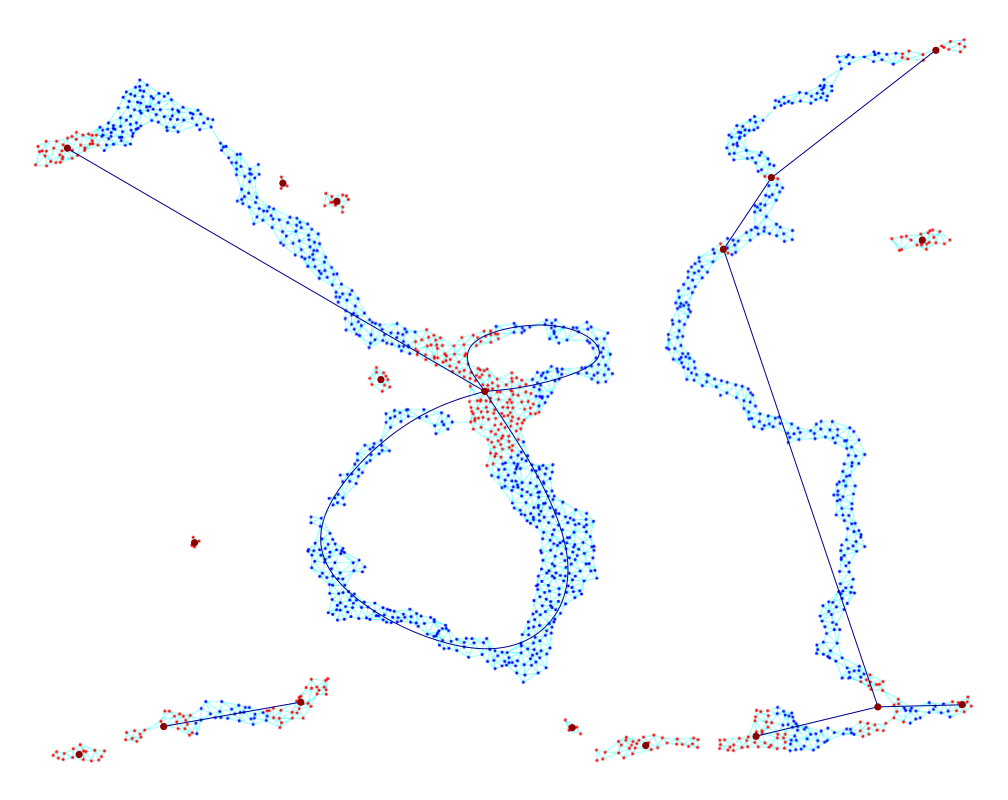
\includegraphics{images/faultlines.png}
\end{figure}
}

\frame{\frametitle{Beispiel (Straßennetz)}
\begin{figure}
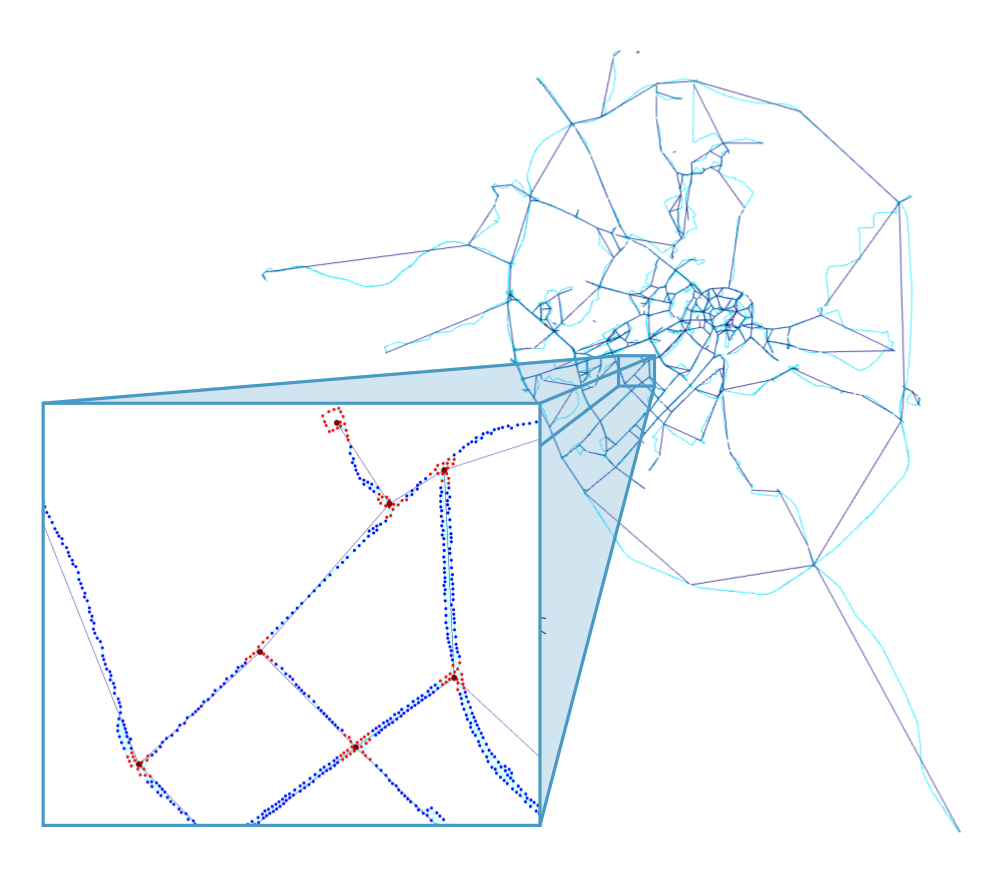
\includegraphics{images/roadnetwork.png}
\end{figure}
}

\frame{\frametitle{Aufgabenbereiche}
  \begin{enumerate}
  \item Vorverarbeitung (Daniel, Terese)
  \item Implementierung des Algorithmus (Lea, Mahmoud, Moritz)
  \item graphische Darstellung der Ergebnisse (Jiang)
  \end{enumerate}
}

\section{Vorverarbeitung}

\frame{\frametitle{Vorverarbeitung}
\begin{enumerate}
\item Menge von Punkten erstellen
  \begin{itemize}
  \item Koordinaten aus GPS-Spur-Dateien extrahieren
  \item Koordinaten der schwarzen Pixel eines Bildes bestimmen
  \end{itemize}
\item ggf. Punktmenge auf repräsentative Teilmenge reduzieren
  \begin{itemize}
  \item metrisches $\varepsilon$-Netz
  \item furthest point sampling
  \end{itemize}
\item auf die Punktmenge basierenden $\alpha$-Komplex erstellen
  \begin{itemize}
  \item $\alpha$-Komplex: Unterkomplex der Delaunay-Triangulierung
  \item nur nahe Punkte werden durch eine Kante verbunden
  \end{itemize}
\item Abstandsmethode implementieren
  \begin{itemize}
  \item $d(x,y) :=$ Länge des kürzesten Pfades zwischen $x$ und $y$
  \end{itemize}
\end{enumerate}
}

\frame{\frametitle{Klassendiagramm}
\begin{figure}
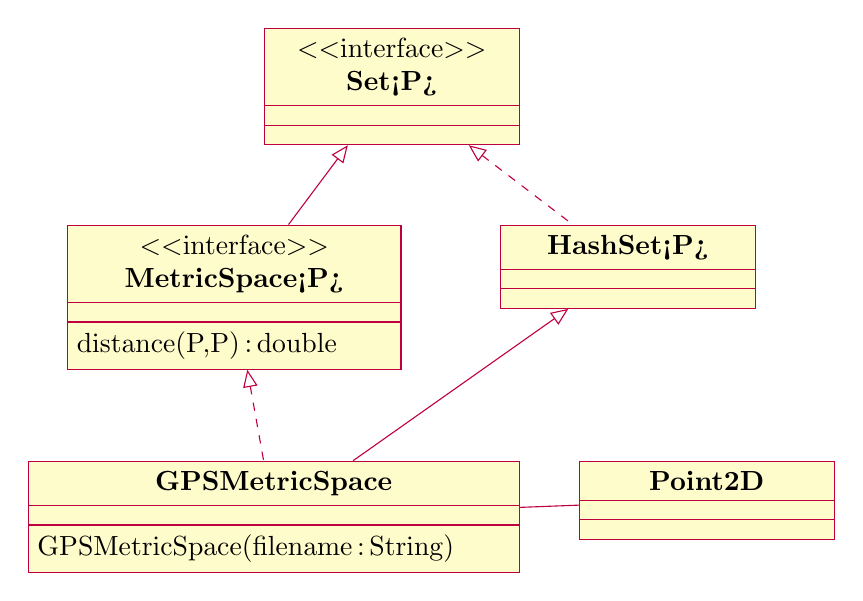
\begin{tikzpicture}
\begin{interface}[text width=3cm]{Set<P>}{0,0}
\end{interface}
\begin{interface}[text width=4cm]{MetricSpace<P>}{-2,-2.5}
\inherit{Set<P>}
\operation{distance(P,P)\,:\,double}
\end{interface}
\begin{class}[text width=3cm]{HashSet<P>}{3,-2.5}
\implement{Set<P>}
\end{class}
\begin{class}[text width=6cm]{GPSMetricSpace}{-1.5,-5.5}
\inherit{HashSet<P>}
\implement{MetricSpace<P>}
\operation{GPSMetricSpace(filename\,:\,String)}
\end{class}
\begin{class}[text width=3cm]{Point2D}{4,-5.5}
\end{class}
\association{Point2D}{}{}{GPSMetricSpace}{}{}
\end{tikzpicture}
\end{figure}
}

\section{Implementierung des Algorithmus}

\subsection{Der Algorithmus}
\frame{\frametitle{Drei wesentliche Schritte}
\begin{enumerate}
	\item[1] Bestimmen, ob Punkte zu Knoten oder Kante im späteren Graphen gehören $\rightarrow$ Punkte mit entsprechendem Label versehen
	\item[2] Anhand der Labels bestimmen, welche Punkte sich zu einem Knoten und welche sich zu einer Kante zusammentun $\rightarrow$ Rekonstruktion des Graphen
	\item[3] Kanten mit Abständen versehen $\rightarrow$ Metrik wiederherstellen
\end{enumerate}
}

\frame{\frametitle{Zu Schritt 1}
\begin{enumerate}
	\item[1] Anhand der Labels bestimmen, welche Punkte sich zu einem Knoten und welche sich zu einer Kante zusammentun $\rightarrow$ Rekonstruktion des Graphen
		\begin{itemize}
			\item Betrachten einen kreisförmigen Ausschnitt um jeden Punkt herum und bestimmen Anzahl der Zusammenhangskomponenten darin
\begin{figure}
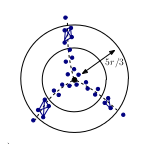
\includegraphics[height=2cm,width=2cm,keepaspectratio]{images/rips1.png}
\end{figure}\pause
			\item Grad des Punkts = Anzahl der Zusammenhangskomponenten im kreisförmigen Ausschnitt\pause
			\item Grad == 2 $\rightarrow$ edge point (wird später zu einer Kante gehören)
			\item Grad != 2 $\rightarrow$ preliminary branch point (wird später zu einem Knoten gehören)
			\item Alle Punkte, die weniger als x von einem primären branch point entfernt sind, werden ebenfalls als branch point eingeordnet
		\end{itemize}
\end{enumerate}
}

\frame{\frametitle{Zu Schritt 2}
\begin{enumerate}
	\item[2] Anhand der Labels bestimmen, welche Punkte sich zu einem Knoten und welche sich zu einer Kante zusammentun $\rightarrow$ Rekonstruktion des Graphen\pause
	\begin{itemize}
		\item Edge und branch points werden in zwei Mengen aufgeteilt 
		\item um die Anzahl der späteren Kanten und Knoten zu bestimmen, wird Rips-Vietoris-Graph erstellt\pause
		\begin{itemize}
			\item Im Rips-Vietoris-Graphen werden alle Punkte, die innerhalb eines gewissen Durchmessers liegen, zu einer Zusammenhangskomponente gefasst 

		\end{itemize}
			\begin{figure}
			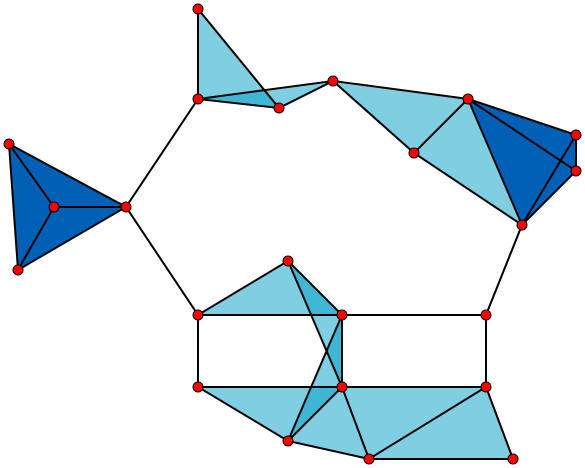
\includegraphics[height=4cm,width=6cm,keepaspectratio]{images/VR_complex.png}
			\end{figure}
		\end{itemize}
\end{enumerate}
}

\frame{\frametitle{Zu Schritt 2}
\begin{enumerate}
	\item[2] Anhand der Labels bestimmen, welche Punkte sich zu einem Knoten und welche sich zu einer Kante zusammentun $\rightarrow$ Rekonstruktion des Graphen
	\begin{itemize}
		\item Edge und branch points werden in zwei Mengen aufgeteilt 
		\item um die Anzahl der späteren Kanten und Knoten zu bestimmen, wird Rips-Vietoris-Graph erstellt\pause
		\item Rips-Vietoris-Graphen für Menge der edge points und Menge der branch points erstellen\pause
		\item Jede Zusammenhangskomponente wird zu einem Knoten, bzw. einer Kante vereint\pause
		\item Zwei Punkte werden durch eine Kante verbunden, wenn sie Punkte in ihrer Zusammenhangskomponente haben, die nur einen gewissen Abstand zu Punkten in der selben Zusammenhangskomponente einer Kante haben
	\end{itemize}
\end{enumerate}
}

\frame{\frametitle{Zu Schritt 3}
\begin{enumerate}
	\item[3] Kanten mit Abständen versehen $\rightarrow$ Metrik wiederherstellen\newline
		\begin{itemize}
		\item Jeder Kante wird als Länge der Durchmesser ihrer Zusammenhangskomponente zugewiesen
	\end{itemize}
\end{enumerate}
}

\subsection{Umsetzung in Java}
\frame{\frametitle{Klassendiagramm}
\begin{figure}
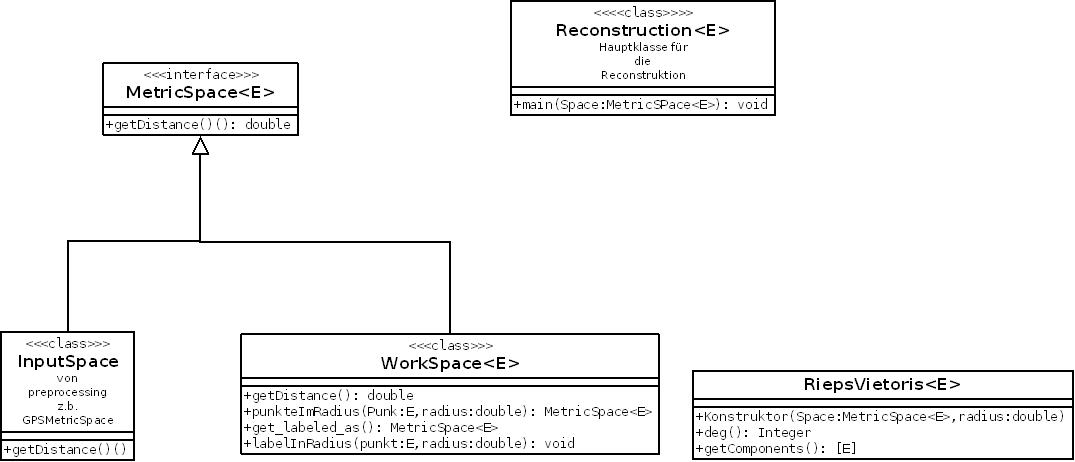
\includegraphics[height=10cm,width=11cm,keepaspectratio]{images/reconstruction_classes.jpeg}
\end{figure}
}

\frame{\frametitle{Verbesserung der Laufzeit}
\begin{itemize}
\item Zunächst naive Implementierung, bis der Algorithmus läuft
\item Dann eventuell Verbesserungen
\begin{itemize}
\item Gitter
\end{itemize}
\end{itemize}
}

\section{Graphische Darstellung der Ergebnisse}

\frame{\frametitle{Graphische Oberfläche}
\begin{itemize}
\item Datei auswählen
  \begin{itemize}
  \item GPS-Spur (GPS Exchange Format [.gpx])
  \item Schwarz-Weiß-Bild (beliebiges Bildformat)
  \end{itemize}
\item Parameter des Algorithmus setzen (?)
\item ursprüngliche Punktmenge wird zusammen mit dem ausgegebenen metrischen Graphen angezeigt
\end{itemize}
}

\frame{\frametitle{Beispiel (Erdbeben)}
\begin{figure}
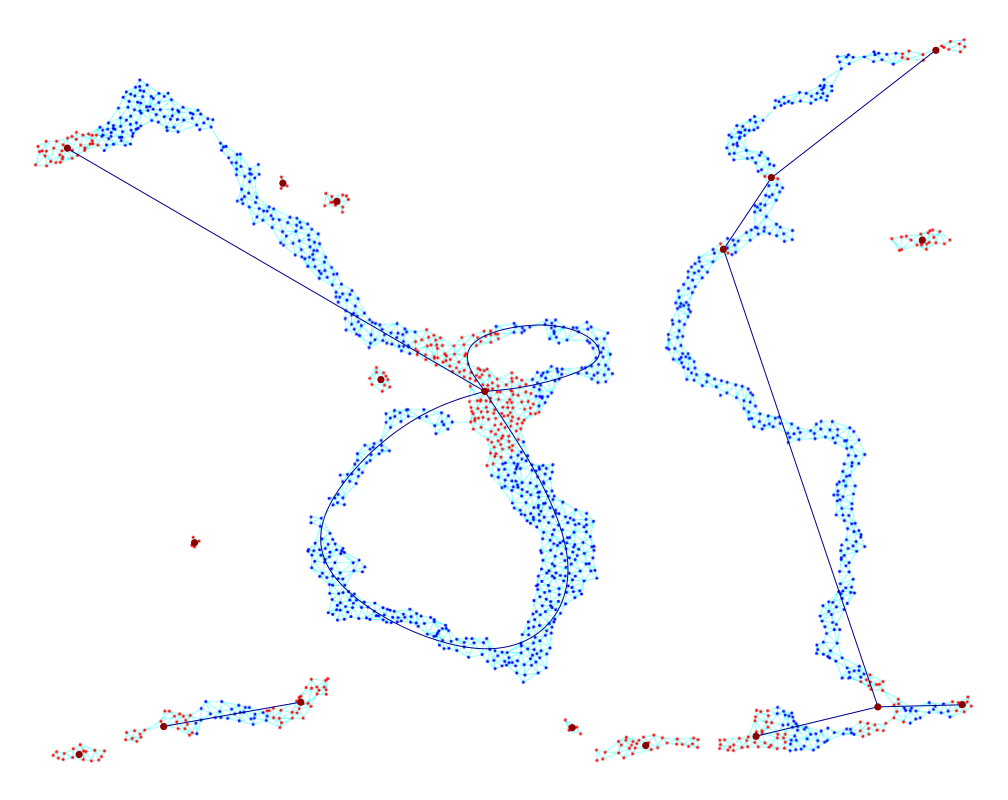
\includegraphics{images/faultlines.png}
\end{figure}
}

\section{Organisation}

\frame{\frametitle{Organisation}
\begin{itemize}
\item Entwicklungsumgebung: Eclipse
\item Versionsverwaltung: Git (in Eclipse integriert)
\item Aufgabenverwaltung: Trello
  \begin{itemize}
  \item zu jeder Aufgabe wird eine Trello-Karte erstellt
  \end{itemize}
\item Dokumentation: Javadoc (und Git Wiki?)
\end{itemize}
}

\frame{\frametitle{Trello}
\begin{figure}
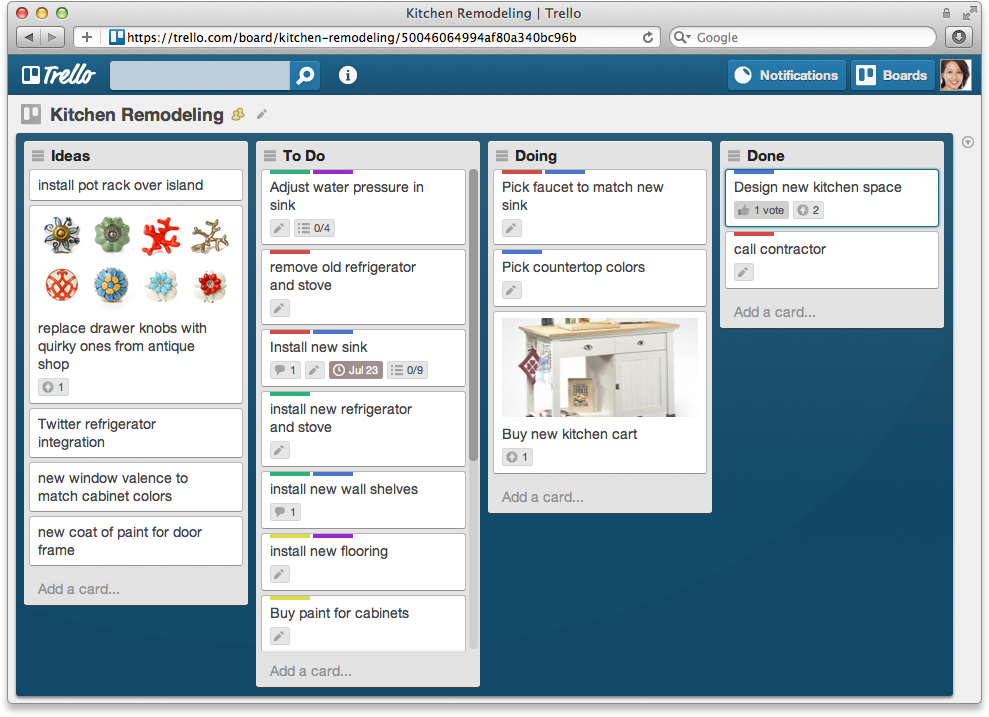
\includegraphics[height=7cm,keepaspectratio]{images/trello.png}
\end{figure}
}

\end{document}
